\documentclass[11pt,letterpaper]{article}
\usepackage[T1]{fontenc}
\usepackage[utf8]{inputenc}
\usepackage[margin=0.75in, top=0.85in, bottom=0.85in]{geometry}
\usepackage[table]{xcolor}
\usepackage{tabularx}
\usepackage{booktabs}
\usepackage{array}
\usepackage{enumitem}
\usepackage{titlesec}
\usepackage{hyperref}
\usepackage{graphicx}
\usepackage{amsmath,amssymb}
\usepackage{fancyhdr}
\usepackage{lastpage}
\usepackage{charter}
\usepackage[scaled=0.92]{helvet}
\usepackage{microtype}
\usepackage[most]{tcolorbox}

% ─────────────────────────────────────────────────────────────
% Color Palette (UMKC Brand & Professional Executive Slate)
% ─────────────────────────────────────────────────────────────
\definecolor{umkcblue}{RGB}{0, 75, 135}       % #004B87 UMKC Primary Blue
\definecolor{umkcgold}{RGB}{218, 165, 32}     % #DAA520 UMKC Gold
\definecolor{headerdark}{RGB}{15, 34, 64}     % #0F2240 Deep Navy
\definecolor{darkslate}{RGB}{30, 41, 59}      % #1E293B Body Text Slate
\definecolor{lightbg}{RGB}{248, 250, 252}     % #F8FAFC Subtle Gray Tint
\definecolor{tableheader}{RGB}{234, 242, 250} % Light Blue Header Fill
\definecolor{bordergray}{RGB}{203, 213, 225}  % Slate 300 Clean Divider
\definecolor{statusgreen}{RGB}{22, 101, 52}   % Forest Green for Completed

% ─────────────────────────────────────────────────────────────
% Hyperlink Setup
% ─────────────────────────────────────────────────────────────
\hypersetup{
    colorlinks=true,
    linkcolor=umkcblue,
    filecolor=umkcblue,
    urlcolor=umkcblue,
    citecolor=umkcblue
}

% ─────────────────────────────────────────────────────────────
% Header and Footer Configuration (fancyhdr)
% ─────────────────────────────────────────────────────────────
\pagestyle{fancy}
\fancyhf{}
\renewcommand{\headrulewidth}{0.5pt}
\renewcommand{\headrule}{\hbox to\headwidth{\color{bordergray}\leaders\hrule height \headrulewidth\hfill}}
\renewcommand{\footrulewidth}{0.5pt}
\renewcommand{\footrule}{\hbox to\headwidth{\color{bordergray}\leaders\hrule height \footrulewidth\hfill}}

\fancyhead[L]{\small\sffamily\textcolor{umkcblue}{\textbf{CS 5551 -- Advanced Software Engineering}}}
\fancyhead[R]{\small\sffamily\textcolor{darkslate}{Team Project: Sprint \#0 Report}}
\fancyfoot[L]{\footnotesize\sffamily\textcolor{darkslate}{Project: \textbf{UMKC Course Timetable Scheduler}}}
\fancyfoot[R]{\footnotesize\sffamily\textcolor{darkslate}{Page \textbf{\thepage} of \textbf{\pageref{LastPage}}}}

% ─────────────────────────────────────────────────────────────
% Section Title Styling
% ─────────────────────────────────────────────────────────────
\titleformat{\section}
  {\Large\bfseries\sffamily\color{headerdark}}
  {\textcolor{umkcblue}{\thesection.}}{0.5em}{}
  [\vspace{-0.3em}{\color{umkcblue}\rule{\textwidth}{1pt}}]

\titlespacing*{\section}{0pt}{14pt}{8pt}

% ─────────────────────────────────────────────────────────────
% Custom Callout Boxes (tcolorbox)
% ─────────────────────────────────────────────────────────────
\tcbset{
    sleekbox/.style={
        colback=lightbg,
        colframe=umkcblue,
        arc=3pt,
        boxrule=0.8pt,
        leftrule=4pt,
        left=10pt,
        right=10pt,
        top=8pt,
        bottom=8pt
    },
    evidencebox/.style={
        colback=white,
        colframe=bordergray,
        arc=4pt,
        boxrule=0.8pt,
        left=8pt,
        right=8pt,
        top=8pt,
        bottom=8pt
    }
}

\begin{document}

% ─────────────────────────────────────────────────────────────
% PAGE 1: TITLE BANNER, OBJECTIVES & STUDENT CONTRIBUTIONS
% ─────────────────────────────────────────────────────────────

% Top Institutional Banner
\begin{center}
    {\LARGE\bfseries\sffamily\color{headerdark} CS 5551 -- Advanced Software Engineering}\\[0.25em]
    {\huge\bfseries\sffamily\color{umkcblue} Team Project: Sprint \#0 Report}\\[0.4em]
    \normalsize\sffamily
    \textbf{Course Instructor:} Dr. Sudipta Chattopadhyay \quad$|$\quad 
    \textbf{Institution:} University of Missouri--Kansas City\\[0.2em]
    \textbf{Submission Date:} September 20, 2026
\end{center}

\vspace{0.4em}

% Objectives & Deliverables Box
\begin{tcolorbox}[sleekbox]
    \sffamily
    \textbf{\color{umkcblue}Objectives:} Report team activities so far and demonstrate that the team has been actively collaborating and accomplishing foundational setup toward completing the first sprint.
    
    \vspace{0.4em}
    \textbf{\color{umkcblue}Deliverables and Grading Policy (Total: 4 points):}
    \begin{enumerate}[topsep=2pt, itemsep=0pt, parsep=2pt, leftmargin=1.8em]
        \item Project Micro-Charter (Brief Description) \textbf{\color{umkcblue}(1 point)}
        \item Meeting Minutes \textbf{\color{umkcblue}(1 point)}
        \item Key Decisions \textbf{\color{umkcblue}(1 point)}
        \item Current Status \textbf{\color{umkcblue}(1 point)}
    \end{enumerate}
\end{tcolorbox}

\vspace{0.3em}
\noindent{\large\bfseries\sffamily\color{headerdark}Report Template}\\[0.2em]
\noindent\small Please use the following template to complete your report. To receive credit for this report, your team must have accomplished some work for the first sprint.

\vspace{0.4em}
\noindent\textbf{Team Name:} {\large\textbf{\color{umkcblue}UMKC Course Timetable Scheduler}}

\vspace{0.4em}
\renewcommand{\arraystretch}{1.3}
\noindent
\begin{tabularx}{\textwidth}{|p{3.2cm}|X|c|c|}
\hline
\rowcolor{tableheader}
\multicolumn{2}{|c|}{\textbf{\sffamily\color{headerdark}Information provided by the student team}} & \multicolumn{2}{c|}{\textbf{\sffamily\color{headerdark}To be used by the grader}} \\ \hline
\rowcolor{tableheader}
\textbf{\sffamily Student name} & \textbf{\sffamily Specific contributions to this sprint} & \textbf{\sffamily Team Score} & \textbf{\sffamily Indiv. Score} \\ \hline
\textbf{Joe Doan} & Project coordination, repository architecture, CI/CD pipeline setup, migration of Google OR-Tools CP-SAT solver engine into monorepo, authoring Sprint 0 onboarding documentation, and verifying 25/25 automated tests. & & \\ \hline
\textbf{Tony Nguyen} & FastAPI backend boilerplate scaffolding, SQLModel relational database entity schema definitions, database connection setup, drafting OpenAPI 3.0 API specification contract, and Pytest test fixtures. & & \\ \hline
\textbf{Tina Nguyen} & Frontend React + Vite + TypeScript initialization, Tailwind CSS design system and theme tokens, application layout shell (Navbar, Sidebar, AppLayout), client-side routing, and Vitest component smoke tests. & & \\ \hline
\textbf{Salvatore Nigro} & FullCalendar library integration and weekly matrix layout, mock timetable dataset schema creation, centralized Axios API service abstraction layer, and TypeScript API contract type definitions. & & \\ \hline
\end{tabularx}

\vspace{0.4em}
\begin{center}
    \textit{\small *A student without specific contributions shall not receive credit.}
\end{center}

\newpage

% ─────────────────────────────────────────────────────────────
% PAGE 2: SECTION 1 - PROJECT MICRO-CHARTER
% ─────────────────────────────────────────────────────────────

\section{Project Micro-Charter}
Provide a brief description of the project, including the following elements:

\begin{itemize}[leftmargin=1.5em, itemsep=5pt, topsep=4pt]
    \item \textbf{Project name:} \textbf{\color{umkcblue}UMKC Course Timetable Scheduler}
    
    \item \textbf{Vision statement:} To deliver an automated, intelligent, and fair course timetabling platform that eliminates multi-week administrative overhead for academic departments, prevents scheduling conflicts, and optimizes faculty teaching satisfaction through mathematical constraint optimization.
    
    \item \textbf{Mission statement / project purpose:} Automate the complex academic course-and-room scheduling workflow for university departments (specifically modeling the UMKC School of Science \& Engineering across 40 courses, 20 instructors, and 12 classrooms) by formulating schedule generation as a Constraint Satisfaction and Optimization Problem (Hard and Soft constraints) powered by Google OR-Tools CP-SAT.
    
    \item \textbf{Elevator pitch:} Traditional university course scheduling is a tedious, error-prone manual process plagued by room double-bookings, capacity overflows, and instructor dissatisfaction. The UMKC Course Timetable Scheduler replaces weeks of ad-hoc negotiation with an automated CP-SAT optimization engine that generates conflict-free, 100\% feasible, multi-semester schedules in seconds while dynamically balancing instructor time preferences, room requirements, and academic rank priority points.
    
    \item \textbf{Customers and users:} 
    \begin{itemize}[itemsep=2pt, topsep=2pt]
        \item \textit{Customers (Decision Makers):} University Academic Leadership (Deans, Department Chairs, Registrar's Office, and Program Directors).
        \item \textit{Users (Direct Actors):} Course Coordinators (who configure constraints, trigger solver runs, and confirm schedules) and Academic Instructors / Faculty Members (who submit time/room preferences, inspect their personalized timetables, and submit schedule adjustment requests).
    \end{itemize}
    
    \item \textbf{Milestones:}
    \begin{itemize}[itemsep=3pt, topsep=2pt]
        \item \textbf{Milestone 0 (Week 5 -- Sprint 0):} Baseline monorepo scaffolding (\texttt{backend/} + \texttt{frontend/}), prototype solver migration with 25 passing test cases, OpenAPI 3.0 contract specification, and CI pipeline setup. \textbf{\color{statusgreen}[Completed]}
        \item \textbf{Milestone 1 (Week 8 -- Sprint 1):} Core relational CRUD APIs (Courses, Rooms, Preferences), Instructor Preference Submission Portal, and Interactive FullCalendar weekly timetable matrix rendering live data.
        \item \textbf{Milestone 2 (Week 12 -- Sprint 2):} Backend API trigger for Google OR-Tools CP-SAT solver, Multi-Semester Simulation engine integration, and Post-Scheduling Edit Request workflow.
        \item \textbf{Milestone 3 (Week 15 -- Sprint 3):} End-to-end integration testing, system containerization (Docker), cloud deployment, user acceptance verification, and final presentation.
    \end{itemize}
    
    \item \textbf{Risks:}
    \begin{itemize}[itemsep=3pt, topsep=2pt]
        \item \textit{Algorithmic Infeasibility / Scalability Risk:} Over-constrained faculty preferences or room capacity deficits could lead to solver timeouts or infeasible solutions. \textbf{Mitigation:} Preprocessing domain validation (\texttt{get\_valid\_ic\_pairs()}), prioritization weighting, soft constraint relaxation, and configurable solver execution deadlines.
        \item \textit{Frontend/Backend API Drift Risk:} Frontend and backend teams building divergent data structures independently. \textbf{Mitigation:} Publishing an authoritative OpenAPI 3.0 YAML specification contract as the single source of truth before feature implementation.
        \item \textit{Team Integration \& Versioning Risk:} Merge conflicts and broken commits across 4 team members. \textbf{Mitigation:} GitHub repository branch protection rules on \texttt{main} and \texttt{dev}, automated CI testing on every pull request, and mandatory peer reviews.
    \end{itemize}
    
    \item \textbf{Authors of this micro-charter:} Joe Doan, Tony Nguyen, Tina Nguyen, Salvatore Nigro.
\end{itemize}

\newpage

% ─────────────────────────────────────────────────────────────
% PAGE 3: SECTION 2 - MEETING MINUTES & EVIDENCE
% ─────────────────────────────────────────────────────────────

\section{Meeting Minutes}
Report the minutes of each meeting. A verified screenshot of the Asana project meeting task card is included below as supporting audit evidence.

\vspace{0.4em}
\renewcommand{\arraystretch}{1.25}
\noindent
\begin{tabularx}{\textwidth}{|p{1.8cm}|p{2.1cm}|p{2.1cm}|p{2.3cm}|X|X|}
\hline
\rowcolor{tableheader}
\textbf{\sffamily Date} & \textbf{\sffamily Time / Dur.} & \textbf{\sffamily Place} & \textbf{\sffamily Participants} & \textbf{\sffamily Purpose of the Meeting} & \textbf{\sffamily Specific Action Items} \\ \hline
09/12/2026 & 2:30 PM -- 3:45 PM (75 min) & Online (Zoom / Discord) & Joe Doan, Tony Nguyen, Tina Nguyen, Salvatore Nigro & First Team Project Meeting: Application logic \& constraints discussion, tech stack confirmation, infrastructure setup, and Sprint 0 action item assignment. & 
1. Discuss Application Logic \& Constraints (Coordinators vs Instructors).\newline
2. Confirm Tech Stack (FastAPI + React, PyTest, Google Style Guide).\newline
3. Infrastructure Setup (GitHub Repo, Teams/Discord, Weekly Meeting).\newline
4. Assign Sprint 0 Action Items \& Schedule Next Meeting. \\ \hline
\end{tabularx}

\vspace{0.8em}
\noindent{\bfseries\sffamily\color{headerdark}Meeting Evidence (Asana Task Card Verification):}

\vspace{0.3em}
\begin{tcolorbox}[evidencebox]
    \centering
    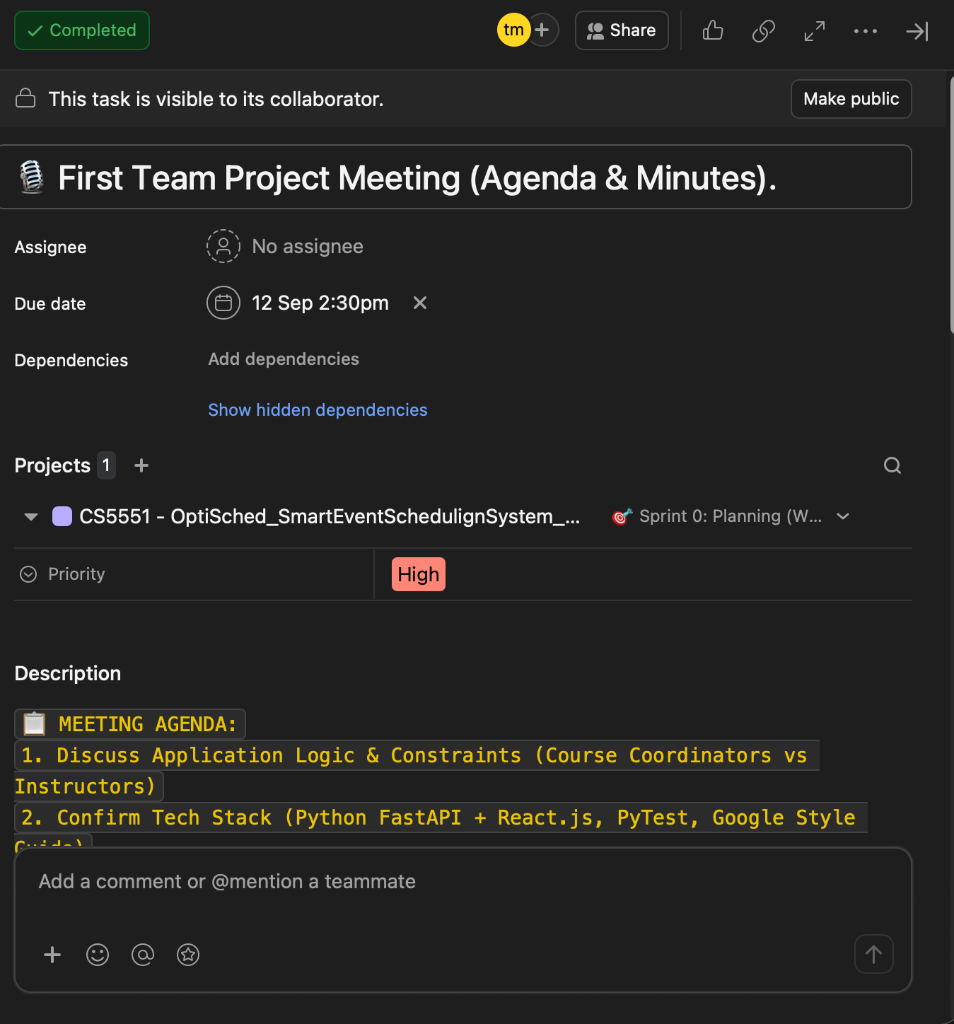
\includegraphics[width=0.68\textwidth, height=6.2cm, keepaspectratio]{meeting1_asana.png}\\[0.4em]
    \small\sffamily
    \textbf{Figure 1:} Verified Asana Task Card --- \textit{First Team Project Meeting (Agenda, Live Minutes \& Action Items)}.\\[0.15em]
    \footnotesize\color{darkslate}
    Asana Project: \textbf{CS5551 -- UMKC Course Timetable Scheduler} $|$ Section: \textbf{Sprint 0: Planning}\\
    Task Status: \textbf{\color{statusgreen}Completed} $|$ Due Date: \textbf{September 12, 2026, 2:30 PM} $|$ Priority: \textbf{High}
\end{tcolorbox}

\vspace{0.4em}
\noindent{\small\bfseries\sffamily\color{headerdark}Meeting Minutes Workflow (via Asana):}
\begin{enumerate}[itemsep=1pt, topsep=2pt, leftmargin=1.8em]
    \small
    \item \textbf{Live Minutes Documentation:} During the meeting, the designated note-taker typed live discussion notes directly into the Asana task card comments section.
    \item \textbf{Action Item Assignment:} Specific subtasks and deadlines were assigned to team members on the Asana Sprint 0 board.
    \item \textbf{Peer Review \& Sign-Off:} Team members reviewed the posted meeting minutes and signified approval via Asana reactions (thumbs up).
    \item \textbf{Formal Completion:} The meeting card was officially marked \textbf{\color{statusgreen}Completed} upon unanimous team concurrence.
\end{enumerate}

\newpage

% ─────────────────────────────────────────────────────────────
% PAGE 4: SECTION 3 - KEY DECISIONS
% ─────────────────────────────────────────────────────────────

\section{Key Decisions \textnormal{\small\textit{(add/delete row only if necessary)}}}

\vspace{0.4em}
\renewcommand{\arraystretch}{1.32}
\noindent
\begin{tabularx}{\textwidth}{|p{4.8cm}|X|}
\hline
\rowcolor{tableheader}
\textbf{\sffamily Decision Item} & \textbf{\sffamily Agreed Selection and Rationale} \\ \hline
\textbf{Programming language and Frameworks} & \textbf{Backend:} Python 3.12 with FastAPI (high performance asynchronous execution, automatic OpenAPI/Swagger documentation generation) and SQLModel ORM.\newline
\textbf{Frontend:} TypeScript with React 18 and Vite (lightning-fast HMR build times, strict end-to-end type safety, component modularity).\newline
\textbf{Optimization Engine:} Google OR-Tools CP-SAT (industry-standard constraint programming solver for NP-hard scheduling). \\ \hline
\textbf{Test framework} & \textbf{Backend:} Pytest, Pytest-Cov, and Python \texttt{unittest} suite.\newline
\textbf{Frontend:} Vitest with React Testing Library and \texttt{jsdom}.\newline
\textbf{CI Pipeline:} GitHub Actions (\texttt{.github/workflows/ci.yml}) executing automated unit and regression suites on every pull request. \\ \hline
\textbf{IDE (Integrated Development Environment)} & Visual Studio Code (standardized with Python, Pylance, ESLint, Prettier, and Tailwind CSS IntelliSense extensions across all team members). \\ \hline
\textbf{Programming style guide} & \textbf{Python:} PEP 8 enforced via \texttt{flake8} and \texttt{black} (line length 88).\newline
\textbf{TypeScript:} ESLint strict configuration paired with Prettier.\newline
\textbf{Git Commits:} Conventional Commits specification (\texttt{feat:}, \texttt{fix:}, \texttt{docs:}, \texttt{test:}, \texttt{chore:}). \\ \hline
\textbf{Project hosting site} & GitHub Repository (Monorepo):\newline
\url{https://github.com/JoeDoan/CS5551_Advanced-Software-Engineering-} \\ \hline
\textbf{Regular meeting time} & Weekly on \textbf{Tuesdays at 2:30 PM CST} (Hybrid format: UMKC Campus in-person collaboration + Discord/Zoom virtual screen-share). \\ \hline
\textbf{Other decisions} & \textbf{Monorepo Architecture:} Unified \texttt{backend/} and \texttt{frontend/} under a single version-controlled repository to guarantee synchronized contracts.\newline
\textbf{Branching Strategy:} Two protected branches (\texttt{main} for stable releases, \texttt{dev} for staging). Individual features developed on \texttt{feature/\textless name\textgreater} with mandatory pull request reviews.\newline
\textbf{Project Management:} Asana Kanban board (To Do, In Progress, In Review, Done) for Sprint backlog tracking, task ownership, and meeting audits. \\ \hline
\end{tabularx}

\newpage

% ─────────────────────────────────────────────────────────────
% PAGE 5: SECTION 4 - CURRENT STATUS & SECTION 5 - BUDDY RATINGS
% ─────────────────────────────────────────────────────────────

\section{Current Status}
Describe how much work is done for each task of Sprint 1 and who has contributed.

\vspace{0.4em}
\renewcommand{\arraystretch}{1.28}
\noindent
\begin{tabularx}{\textwidth}{|p{3.4cm}|X|p{4.2cm}|}
\hline
\rowcolor{tableheader}
\textbf{\sffamily Task} & \textbf{\sffamily What Is Done} & \textbf{\sffamily Who Has Contributed} \\ \hline
\textbf{User stories} & Authored comprehensive user stories for Sprint 1 spanning both Course Coordinator (e.g., viewing master schedule matrix, room allocation) and Instructor personas (e.g., submitting day/time preferences, viewing personal timetable). Stored in Asana backlog. & Joe Doan, Tony Nguyen, Tina Nguyen, Salvatore Nigro \\ \hline
\textbf{Acceptance criteria} & Defined rigorous Given-When-Then acceptance criteria for Sprint 1: zero room double-booking validation, maximum 2 courses per faculty enforcement, successful \texttt{/health} HTTP 200 response, and FullCalendar weekday rendering. & Joe Doan, Tony Nguyen \\ \hline
\textbf{Coding (optional)} & \textbf{1. Monorepo Scaffolding:} Configured root workspace, environment files, and GitHub Actions CI workflow.\newline
\textbf{2. Solver Migration:} Integrated Google OR-Tools CP-SAT engine into \texttt{backend/app/solver/} with \textbf{25/25 verification tests passing 100\%}.\newline
\textbf{3. Backend Architecture:} Built FastAPI entrypoint, SQLModel relational entities, and drafted OpenAPI 3.0 contract specification.\newline
\textbf{4. Frontend Architecture:} Initialized React+Vite+Tailwind shell with responsive Navbar, Sidebar, routes, and FullCalendar timetable skeleton. & 
\textbf{Joe Doan} (Solver engine, DevOps, CI pipeline)\newline
\textbf{Tony Nguyen} (FastAPI, SQLModel, OpenAPI spec)\newline
\textbf{Tina Nguyen} (React layout shell, routing, Tailwind)\newline
\textbf{Salvatore Nigro} (FullCalendar skeleton, API client) \\ \hline
\end{tabularx}

\vspace{1.0em}

\section{Buddy Ratings \textnormal{\small\textit{(add/delete row if necessary)}}}
If you don't feel comfortable to include your ratings in this report, you may email your ratings to the instructor or grader.

\vspace{0.4em}
\renewcommand{\arraystretch}{1.25}
\noindent
\begin{tabularx}{\textwidth}{|l|c|c|c|c|}
\hline
\rowcolor{tableheader}
\multicolumn{5}{|c|}{\textbf{\sffamily Rating receiver}} \\ \hline
\rowcolor{tableheader}
\textbf{\sffamily Rating giver} & \textbf{\sffamily Joe Doan} & \textbf{\sffamily Tony Nguyen} & \textbf{\sffamily Tina Nguyen} & \textbf{\sffamily Salvatore Nigro} \\ \hline
\textbf{Joe Doan} & \cellcolor{gray!15}\textbf{X} & 1.0 & 1.0 & 1.0 \\ \hline
\textbf{Tony Nguyen} & 1.0 & \cellcolor{gray!15}\textbf{X} & 1.0 & 1.0 \\ \hline
\textbf{Tina Nguyen} & 1.0 & 1.0 & \cellcolor{gray!15}\textbf{X} & 1.0 \\ \hline
\textbf{Salvatore Nigro} & 1.0 & 1.0 & 1.0 & \cellcolor{gray!15}\textbf{X} \\ \hline
\rowcolor{tableheader}
\textbf{\sffamily Average} & \textbf{1.0} & \textbf{1.0} & \textbf{1.0} & \textbf{1.0} \\ \hline
\end{tabularx}

\vspace{2.0em}
\begin{center}
    {\color{bordergray}\rule{0.6\textwidth}{0.6pt}}\\[0.5em]
    \textit{\small\sffamily\textcolor{darkslate}{End of Sprint \#0 Report --- CS 5551 Advanced Software Engineering --- School of Science \& Engineering, UMKC}}
\end{center}

\end{document}
